% This is samplepaper.tex, a sample chapter demonstrating the
% LLNCS macro package for Springer Computer Science proceedings;
% Version 2.20 of 2017/10/04
%
\documentclass[runningheads]{llncs}
%
\usepackage{amsmath}
\usepackage{graphicx}
\usepackage{chngpage}
% Used for displaying a sample figure. If possible, figure files should
% be included in EPS format.
%
% If you use the hyperref package, please uncomment the following line
% to display URLs in blue roman font according to Springer's eBook style:
% \renewcommand\UrlFont{\color{blue}\rmfamily}

\begin{document}
%
\title{Clasificación binaria y multiclase mediante Regresión logística}
%
%\titlerunning{Abbreviated paper title}
% If the paper title is too long for the running head, you can set
% an abbreviated paper title here
%
\author{Eguiarte Morett Luis Andrés \and Ortiz Barajas Jesús Germán}
%

% First names are abbreviated in the running head.
% If there are more than two authors, 'et al.' is used.
%
\institute{Instituto de Investigaciones en Matemáticas Aplicadas y en Sistemas (IIMAS) \\Universidad Nacional Autóonoma de México (UNAM)}
%
\maketitle              % typeset the header of the contribution
%
\begin{abstract}
En el presente trabajo, se perseguirá aplicar métodos de aprendizaje supervisado en el problema de clasificación de un conjunto de datos representativo de canciones pertenecientes a un par de géneros musicales, en específico Rock y Hip-Hop. Iremos desde la preparación, limpieza y análisis de los datos para poder utilizarlos, hasta el entrenamiento de un par de modelos, en específico regresión logística y árboles de decisión, pasando por normalización, reducción de dimensionalidad para evitar redundancia de características y un balanceo de los datos para mejorar los clasificadores. La utilización de arboles de decisión tiene como fin poder establecer una comparativa de las métricas de clasificación arrojadas a la hora de evaluar los modelos. Posteriormente, procederemos a mostrar los resultados obtenidos utilizando una implementación propia de regresión logística. Veremos que nuestra implementación de regresión logística obtiene los mismos resultados que la implementación en la popular biblioteca $scikitlearn$, y que presenta mejoras en cuanto a tiempo de ejecución utilizando el mismo optimizador que utiliza por defecto la regresión logística en la biblioteca $scikitlearn$ (L-BFGS). También presentaremos a detalle el modelo de regresión logística utilizado para nuestra implementación, que fue tanto multiclase, como únicamente de dos clases, su vectorización y paralelización para el caso de más de dos clases. Continuaremos mostrando tiempos de ejecución para tanto la versión serial como paralela de la regresión logística multiclase, que en este caso será probada con el conocido MNIST dataset \cite{Dua:2019}, y observaremos que mientras la versión serial sigue teniendo una ventaja contra la implementación de $scikitlearn$, nuestra implementación concurrente presenta cuellos de botella, para los cuales hipotetizaremos sobre las causas. Finalizaremos haciendo pruebas de ejecución con Dask y Numba.

\end{abstract}

\section{Introducción}
Los sistemas de aprendizaje de máquina se dividen de acuerdo a la cantidad y tipo de supervisión que reciben durante su entrenamiento en: aprendizaje supervisado, no supervisado, semi-supervisado y por reforzamiento \cite{handsonML}. El aprendizaje supervisado trata con conjuntos de datos etiquetados previamente, mientras que el aprendizaje no supervisado intenta "encontrar" estas etiquetas, el aprendizaje por reforzamiento intenta entrenar agentes con base en una retroalimentación entre estímulo del entorno y respuesta del agente, encontrando la mejor respuesta a los estímulos. Dentro del aprendizaje supervisado, se encuentran los métodos de clasificación, los cuales tratan con conjuntos de datos donde las etiquetas indican pertenencia a cierto conjunto, la idea principal es entrenar a un modelo con estos datos previamente etiquetados para que éste pueda posteriormente predecir o reconocer correctamente la clase a la que pertenece cierto ejemplo. Sin embargo, entrenar un modelo de aprendizaje supervisado con un conjunto de datos etiquetado, la mayoría del tiempo no es una tarea trivial, y presenta diversas dificultades que exigen ser mitigadas mediante análisis previos, limpieza, preparación y otra serie de técnicas que nos ayuden a mejorar la calidad del modelo.

\section{Conjunto de datos}
En esta sección describimos los dos conjuntos de datos utilizados para la realización de experimentos con árboles de decisión y regresión logística, tanto la implementación de la biblioteca \textit{scikit-learn} como la implementación propia.

\subsection{Digitos escritos a mano}
En primer lugar, utilizamos una versión del \textit{Pen-Based Recognition of Handwritten Digits Data Set} \cite{Dua:2019} disponible en la biblioteca \textit{sci-kit learn}\footnote{https://scikit-learn.org/stable/auto\_examples/datasets/plot\_digits\_last\_image.html}, el cual consta de 1797 imágenes de $8 \times 8$ de digitos escritos a mano que van desde el 0 al 9, cada uno etiquetado con digito al que pertenecen, es decir, el conjunto de datos tiene 10 etiquetas, correspondientes a los digitos 0 al 9. La figura \ref{fig:digitsExample} muestra un ejemplo de las imágenes del conjunto de datos, con dígitos que van del cero al tres.

\begin{figure}[h]
    \centering
    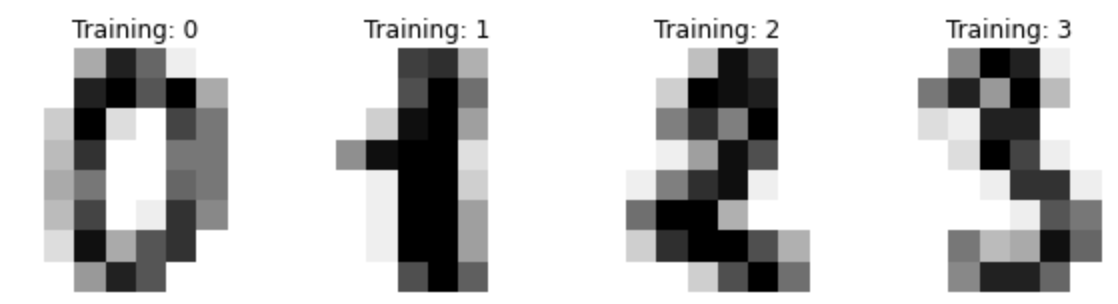
\includegraphics[scale=0.4]{img/digits.png}
    \caption{Ejemplo de datos del \textit{Pen-Based Recognition of Handwritten Digits Data Set}}
    \label{fig:digitsExample}
\end{figure}

\subsection{Géneros musicales}
En segundo lugar, utilizamos un conjunto de datos de información múscial correspondiente a dos géneros musicales: rock y hip-hop; el cual consta de 4802 canciones, de las cuales se tienen las características acústica, bailabilidad, energía, instrumentalidad, vivacidad, habla, tempo y  valencia. De estas instancias, 3892 están etiquetadas con el género rock, mientas que 910 corresponden a la etiqueta Hip-hop. El conjunto de datos está disponible en los proyectos del sitio web \textit{Datacamp}\footnote{https://learn.datacamp.com/projects/449}. La tabla \ref{tab:conjuntoMusica} muestra 10 instancias del conjunto de datos de información musical.

\begin{table}[h]
    \centering
    \begin{adjustwidth}{-.5in}{-.5in}
    \begin{tabular}{|c|c|c|c|c|c|c|c|c|c|}
    \hline
    track\_id & acústica & bailabilidad & energía & instrumentalidad & vivacidad & habla & tempo & valencia & género \\
    \hline
    2 & 0.416675 & 0.675894 & 0.634476 & 0.010628 & 0.177647 & 0.159310 & 165.922 & 0.576661 & Hip-Hop \\
    3 & 0.374408 & 0.528643 & 0.817461 & 0.001851 & 0.105880 & 0.461818 & 126.957 & 0.269240 & Hip-Hop \\
    5 & 0.043567 & 0.745566 & 0.701470 & 0.000697 & 0.373143 & 0.124595 & 100.260 & 0.621661 & Hip-Hop \\
    134 & 0.452217 & 0.513238 & 0.560410 & 0.019443 & 0.096567 & 0.525519 & 114.290 & 0.894072 & Hip-Hop \\
    153 & 0.988306 & 0.255661 & 0.979774 & 0.973006 & 0.121342 & 0.051740 & 90.241 & 0.034018 & Rock \\
    154 & 0.970135 & 0.352946 & 0.023852 & 0.957113 & 0.113261 & 0.032177 & 53.758 & 0.035632 & Rock \\
    155 & 0.981657 & 0.142249 & 0.912122 & 0.967294 & 0.363510 & 0.087527 & 91.912 & 0.034325 & Rock \\
    169 & 0.989141 & 0.225978 & 0.722835 & 0.263076 & 0.092371 & 0.053406 & 94.322 & 0.028347 & Rock \\
    170 & 0.886660 & 0.298518 & 0.744333 & 0.920950 & 0.139587 & 0.088781 & 97.880 & 0.073548 & Rock \\
    171 & 0.698278 & 0.285816 & 0.213494 & 0.955691 & 0.087036 & 0.064094 & 125.645 & 0.150599 & Rock \\
    \hline
    \end{tabular}
    \end{adjustwidth}
    \caption{Intancias del conjunto de datos de información musical}
    \label{tab:conjuntoMusica}
\end{table}

\section{Metodología}
En esta sección describimos el preprocesamiento realizado sobre los conjuntos de datos, los clasificadores utilizados, los detalles de la implementación de regresión logística propuesta, las herramientas utilizadas para el mejoramiento del rendimiento de los clasificadores, así como los experimentos realizados.

\subsection{Preprocesamiento de datos}\label{subsec:Preproc}
Antes de alimentar los algoritmos de aprendizaje de máquina, llevamos a cabo un preprocesamiento para ambos conjuntos de datos, a continuación se describe cada uno de ellos.
\subsubsection{Géneros musicales}
En primer lugar, se obtuvo una matriz de correlación entre las variables. La matriz de correlación es una matriz cuadrada ($K \times K$) y simétrica cuya posición $P_{ij}$ es la correlación entre las columnas i y j del conjunto de datos \cite{Brown2009ComprehensiveCS}. En términos simples, indica cuanto cambia una variable cuando otra variable cambia. La figura \ref{fig:corrMatrix} muestra la matriz de correlación de las características del conjunto de datos de información musical.

\begin{figure}[h]
    \centering
    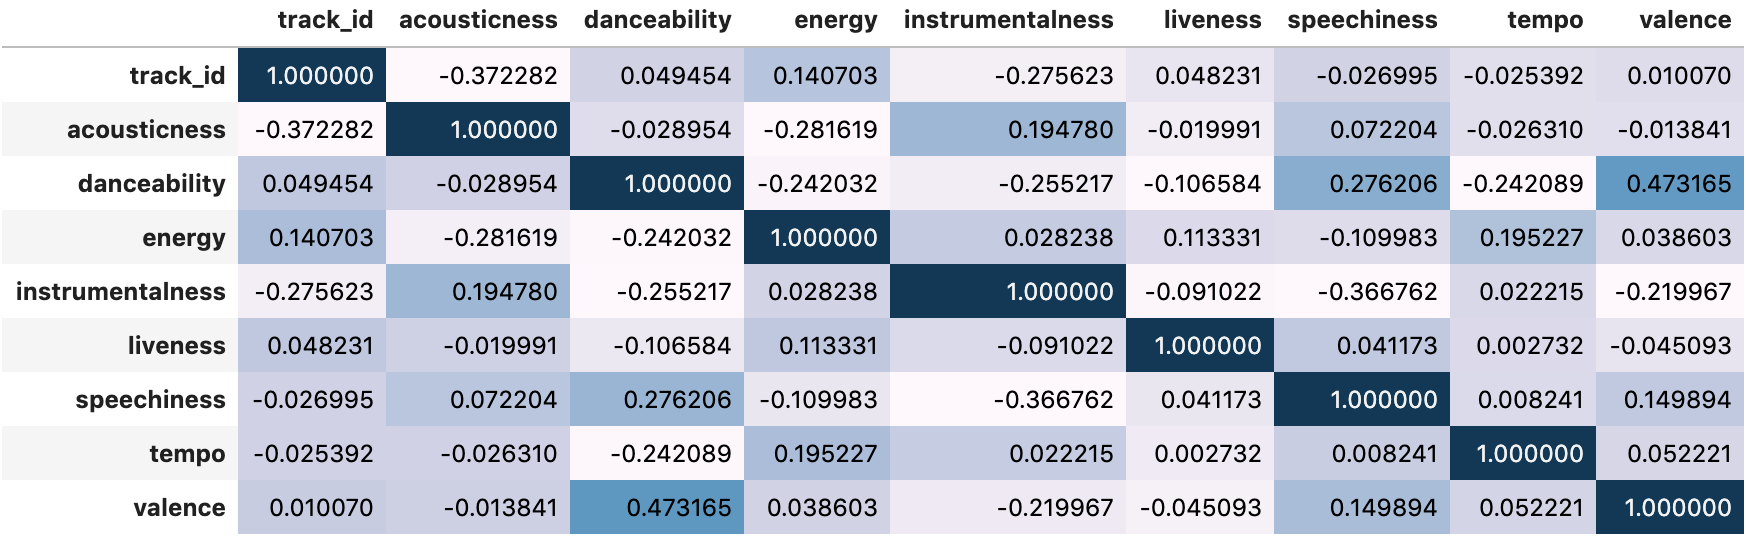
\includegraphics[scale=0.35]{img/corrMatrix.png}
    \caption{Matriz de correlación para el conjunto de datos de información musical}
    \label{fig:corrMatrix}
\end{figure}

Después de observar que no existe una fuerte correlación entre las variables, realizamos una normalización de los datos mediante el algoritmo \textit{StandardScaler}, el cual  elimina la media de los datos y escala los datos de forma que su varianza sea igual a 1. Posteriormente, llevamos a cabo una reducción de dimensionalidad, mediante el algoritmo de Análisis de Componentes Principales (PCA)\cite{pca}, el cual consiste en buscar combinaciones lineales de las variables originales que representen lo mejor posible a la variabilidad presente en los datos de forma que con estas combinaciones lineales, que serán los componentes principales, sea suficiente para representar de manera correcta la información contenida en los datos. Para determinar el número de componentes principales a considerar utilizamos la gráfica de gráfica de varianza explicada acumulada y seleccionamos el número de componentes el 0.9 de varianza explicada acumulada. Para el caso del conjunto de datos de información músical, realizamos la reducción a 6 componentes. La figura \ref{fig:cumulativeVariance} muestra la gráfica de varianza explicada acumulada, donde se observa que el número de componentes que excede el valor de 0.9 es igual a 6.

\begin{figure}[h]
    \centering
    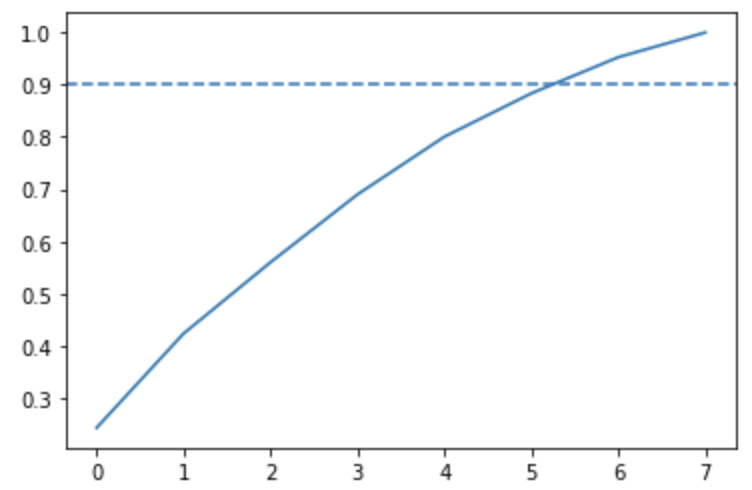
\includegraphics[scale=0.6]{img/cumulativeVariance.png}
    \caption{Gráfica de varianza explicada acumulada}
    \label{fig:cumulativeVariance}
\end{figure}

\subsubsection{Digitos escritos a mano}
Dado que este conjunto de datos está diseñado específicamente para realizar experimentos sobre el directamente, ningún preprocesamiento se llevó a cabo sobre este conjunto de datos. 

\subsection{Clasificador}
El algoritmo que se implementará como clasificador es la regresión logística; lo que hace este algoritmo es estimar la probabilidad de que una instancia pertenezca a una clase particular. Si la probabilidad estimada es superior al 50\%, el modelo predice que la instancia pertenece a una clase i , en caso contrario predice que la instancia pertenece a la clase j. Este caso binario puede extenderse a un problema multiclase si se realiza este procedimiento para cada una de las clases que componen el conjunto de datos \cite{handsonML}.

Para el problema de clasificación binaria, se tiene que:
\begin{equation}
    y \in \{0,1\}
\end{equation}
Mientras que para la clasificación multiclase:
\begin{equation}
    y \in \{0,1,2,..., i, ..., c - 1\}
    \label{eqn:multiclase}
\end{equation}

\noindent
Al igual que en la regresión lineal, calcula una suma ponderada de las características de entrada junto con un término de sesgo:
\begin{equation}
    z = \theta^{T}x = \sum_{j=0}^{n}\theta_jx_j
\end{equation}
Donde:
\begin{equation}
    x = \begin{bmatrix}
           x_{0} \\
           x_{1} \\
           \vdots \\
           x_{n}
         \end{bmatrix}
\end{equation}
y
\begin{equation}
    \theta = \begin{bmatrix}
           \theta_{0} \\
           \theta_{1} \\
           \vdots \\
           \theta_{n}
         \end{bmatrix}
\end{equation}
Para representar el término de bias o sesgo, i.e. el término $\theta_0$ independiente, se hace $x_0 = 1$, además cabe hacer notar que $n$ es el número de características o features por instancia del dataset, es decir, es la dimensión de nuestro vector de características $x$ y por ende, la dimensión del vector de parámetros $\theta$, si contamos el término de sesgo que necesita el modelo, tendremos que ambos vectores son de dimensión $n + 1$.\\
En general, un modelo de aprendizaje supervisado tiene como objetivo ajustar una función de hipótesis $h_{\theta}$, mediante un algoritmo de aprendizaje y un conjunto de datos de entrenamiento. Por ejemplo para la regresión lineal, la función de hipótesis es:
\begin{equation}
    h_{\theta}(x) = z = \theta^{T}x
\end{equation}

Para el caso de la regresión logística, en lugar de generar el resultado directamente como lo hace el modelo de regresión lineal, la salida es la función logística de este resultado como se muestra en la ecuación (\ref{eqn:EstimatedProbability}), que se puede interpretar como  la probabilidad de que $y = 1$, dada $x$, parametrizada por $\theta$, la cual cubriría el caso de la regresión logística de dos clases. Esta función logística es la función sigmoide, la cual genera un número entre cero y uno, y se define como se muestra en la ecuación \ref{eqn:LogisticFunction}.

\begin{equation}
    \hat{p}(y = 1| x;\theta) = h_{\theta}(x) = g(\theta^{T}x)
    \label{eqn:EstimatedProbability}
\end{equation}


\begin{equation}
    g(z) = \frac{1}{1 + e^{-z}}
    \label{eqn:LogisticFunction}
\end{equation}

Gracias a esta función $g$, podremos realizar clasificaciones multiclase, lo cuál es un ventaja frente a una regresión lineal estándar, la cual únicamente puede utilizarse como clasificador de dos clases.\\
Una vez definida la función de hipótesis, debemos definir una función de costo para entrenar a nuestro modelo, como en gran cantidad de modelos de aprendizaje supervisado, este función será la suma del error cuadrático medio entre los valores que nuestro modelo o hipótesis estima $h_{\theta}(x)$ para cada ejemplo y los valores reales con los cuales está etiquetado cada ejemplo $y$.
\begin{equation}
    J(\theta) = \frac{1}{m}\sum_{i = 1}^{m}(\frac{1}{2}h_{\theta}(x^{(i)}) - y^{(i)})^2
    \label{eqn:CostFunction}
\end{equation}
Para la ecuación anterior, los superíndices no representan potencias, sino renglones dentro de la matriz del dataset.\\
Una vez que tenemos definida la función de costo podríamos aplicar el algoritmo de descenso del gradiente, para encontrar su mínimo, sin embargo, no podemos aplicarlo directamente en (\ref{eqn:CostFunction}) puesto que nuestra función de hipótesis al ser no lineal, provocará que tengamos una función de costo no convexa, y que por lo tanto será susceptible a que al aplicar el descenso del gradiente directamente (y cualquier otro algoritmo de optimización basado en gradiente) pueda quedarse atrapado en mínimos locales. Para resolver esto vamos definir una nueva norma, de manera tal que la nueva función de costo, nos codifique el hecho de que sea cero si $y = 1$ para $\hat{p}(y = 1| x;\theta)$ o si $y = 0$ para $\hat{p}(y = 0| x;\theta)$
\begin{equation}
    costo_{\theta}(h_{\theta}(x), y) = \begin{cases} 
      -\log(h_{\theta}(x)) & y = 1 \\
      -\log(1 - h_{\theta}(x)) & y = 0
   \end{cases}
\end{equation}
Que se puede reescribir de la forma:
\begin{equation}
    costo_{\theta}(h_{\theta}(x), y) = -y\log(h_{\theta}(x)) - (1 - y)\log(1 - h_{\theta}(x))
    \label{eqn:CostLog}
\end{equation}
Si ahora definimos (\ref{eqn:CostFunction}) como:
\begin{equation}
    J(\theta) = \frac{1}{m}\sum_{i = 1}^{m}costo_{\theta}(h_{\theta}(x), y)
    \label{eqn:CostFunctionLog}
\end{equation}
Sustituyendo (\ref{eqn:CostLog}) en (\ref{eqn:CostFunctionLog}):
\begin{equation}
    J(\theta) = -\frac{1}{m}\sum_{i = 1}^{m}(y^{(i)}\log(h_{\theta}(x^{(i)})) + (1 - y^{(i)})\log(1 - h_{\theta}(x^{(i)})))
    \label{eqn:CostFunctionLogistic}
\end{equation}
La función expresada en (\ref{eqn:CostFunctionLogistic}) es convexa, es decir, tiene un mínimo global, si calculamos su gradiente, ya podremos utilizar el resultado de este cálculo para entrenar el modelo de regresión logística ya sea con descenso del gradiente o cualquier otro método numérico de optimización de funciones basado en gradientes.\\
Calculando el gradiente de (\ref{eqn:CostFunctionLogistic}) y expresándolo en notación indicial nos quedará que:
\begin{equation}
    \frac{\partial J(\theta_j)}{\partial\theta_j } = \frac{1}{m}\sum_{i = 1}^{m}(h_{\theta}(x^{(i)}) - y^{(i)})x_j^{(i)}
    \label{eqn:DerivCostFunction}
\end{equation}
Además, para hacer nuestro modelo menos susceptible al sobreajuste (overfitting) por tener demasiadas características, vamos introducir un término para la regularización de las características. Con la introducción de este término, vamos a poder mantener todas las características, simplemente se reducirá la magnitud de todas las características, haciendo que las características que influyan poco en la predicción sean penalizadas. Introduciendo el término de regularización, las expresiones (\ref{eqn:CostFunctionLogistic}) y  (\ref{eqn:DerivCostFunction}) quedan:
\begin{equation}
        J(\theta) = -\frac{1}{m}\sum_{i = 1}^{m}(y^{(i)}\log(h_{\theta}(x^{(i)})) + (1 - y^{(i)})\log(1 - h_{\theta}(x^{(i)}))) + \frac{\lambda}{2m}\sum_{j = 1}^{n}\theta_j^2
    \label{eqn:CostFunctionLogisticReg}
\end{equation}
\begin{equation}
        \frac{\partial J(\theta_j)}{\partial\theta_j } = \frac{1}{m}\sum_{i = 1}^{m}(h_{\theta}(x^{(i)}) - y^{(i)})x_j^{(i)} + \frac{\lambda}{m}\theta_j
    \label{eqn:DerivCostFunctionReg}
\end{equation}
Donde $\lambda$ es el parámetro de regularización.\cite{MLCoursera}\\
Este par de funciones se podrían implementar directamente, sin embargo conllevarían hacer dos ciclos for anidados, o bien, en una implementación parcialmente vectorizada, se podría hacer en un solo ciclo for. Vamos a vectorizar completamente estas dos expresiones, es decir, las vamos a expresar en forma vectorial matricial, de manera tal que a la hora de implementarlas únicamente tendremos que valernos de estas expresiones operando directamente sobre matrices y vectores de $numpy$.\\
Las expresiones (\ref{eqn:CostFunctionLogisticReg}) y (\ref{eqn:DerivCostFunctionReg}) se pueden expresar de forma vectorial matricial como:
\begin{equation}
        J(\theta) = \frac{1}{m}(-y^T\log(h_{\theta}(X\Theta)) - (1 - y)^T\log(1 - h_{\theta}(X\Theta))) + \frac{\lambda}{2m}(I'\Theta^T\Theta)
    \label{eqn:CostFunctionLogisticReg}
\end{equation}
\begin{equation}
        \nabla\Theta = \frac{1}{m}X^T(h_{\theta}(X\Theta) - y) + \frac{\lambda}{m}I'\Theta
    \label{eqn:DerivCostFunctionReg}
\end{equation}
Donde:
\begin{equation}
    I'_{ij} = \begin{cases}
        1 & i = j \neq 0 \\
        0 & i \neq j \\
        0 & i = j = 0
    \end{cases}
\end{equation}
Estas dos funciones se pasarán como parámetros a la función de optimización de $optimize.fmin\_l\_bfgs\_b$ de $scikitlearn$, la implementación del algoritmo de optimización de funciones escalares $L-BFGS$ de dicha biblioteca, con la cuál se efectuará el entrenamiento del modelo, puesto que precisamente es un algoritmo de optimización de funciones basado en el gradiente \cite{NoceWrig06}.\\
\noindent
Para la regresión logística multiclase utilizaremos un paradigma uno vs. todos, con base en (\ref{eqn:multiclase}):
\begin{equation}
    \begin{cases}
        h_{\theta}^{(0)} = \hat{p}(y = 0|x;\theta)\\
        h_{\theta}^{(1)} = \hat{p}(y = 1|x;\theta)\\
        \vdots\\
        h_{\theta}^{(c - 1)} = \hat{p}(y = c - 1|x;\theta)
    \end{cases}
\end{equation}
Es decir, para cada clase, tendremos un modelo de clasificación, cada modelo separa una clase de las demás, de manera tal que para predecir a que clase pertenece un ejemplo, tomaremos el modelo que regrese el valor más alto \cite{MLCoursera}:
\begin{equation}
    prediccion = max_i(h_{\theta}^{(i)}(x^{(j)}))
\end{equation}
Como podemos ver, cada modelo de regresión logística de cada clase, es completamente independiente en su entrenamiento de los demás modelos, por lo tanto, bajo nuestro planteamiento de regresión logística multiclase, podríamos paralelizar el entrenamiento de varios modelos a la vez ya sea en varios procesos o en varios hilos, esto fue precisamente lo que se intentó, sin embargo no se observó gran mejora ni respecto a la ejecución en serie propia, ni respecto a la ejecución de la implementación de la regresión logística de $scikitlearn$, $sklearn.linear\_model.LogisticRegression$ con el parámetro $n\_jobs > 1$, es decir, en paralelo.


Para el desarrollo de este proyecto comparamos tres implementaciones distintas del algoritmo de regresión logística, la primera, utilizando la biblioteca \textit{Sci-kit learn}, en segundo lugar, utilizando la biblioteca \textit{Dask} y finalmente una implementación desarrollada por nosotros.

Para el caso del problema de clasificación de géneros musicales para cada una de las implementaciones descritas anteriormente, tomamos en cuenta distintas variantes, de las cuales medimos el tiempo de ejecución mediante la biblioteca \textit{timeit} disponible en Python.

Para el caso de la implementación de \textit{Sci-kit learn}, realizamos experimentos con los parámetros por defecto que ofrece la biblioteca y utilizando como \textit{backend} el ofrecido por la biblioteca \textit{Dask} \cite{dask}. Esta biblioteca permite la computación en paralelo. Combina algoritmos de bloque con programación de tareas dinámica para lograr un clon de la biblioteca \textit{NumPy} \cite{harris2020array} pero que trabaja en paralelo. El \textit{backend} de Dask permite entrenar modelos de aprendizaje automático usando todos los núcleos de un clúster sin la necesidad de realizar cambios significativos en el código.

Por otra parte, para probar la implementación de la biblioteca \textit{Dask} realizamos llevamos a cabo todo el procedimiento descrito en la sección \ref{subsec:Preproc} utilizando las funciones de dicha biblioteca, que permiten la paralelización de tareas.

Finalmente, para la experimentación utilizando la implementación propia del algoritmo de regresión logística, implementada con las bibliotecas \textit{NumPy} y \textit{SciPy}, realizamos pruebas utilizando la biblioteca \textit{Numba} \cite{10.1145/2833157.2833162}, la cual permite traducir código de Python a código máquina, a partir de cambios sencillos en el código mediante el uso de decoradores.


\subsection{Configuración experimental}
Todos los experimentos fueron llevados a cabo en el lenguaje de programación Python mediante cuadernos de \textit{Jupyter}. Para el entrenamiento y prueba de los algoritmos, dividimos el conjunto de datos en conjuntos de entrenamiento y prueba, con tamaños del 75\% y 25\% respectivamente. Para medir el rendimiento de las implementaciones y variaciones consideradas en función del tiempo de ejecución, usamos la biblioteca \textit{Timeit}, finalmente para medir el rendimiento del clasificador, utilizamos las métricas \textit{Accuracy}, \textit{Precision}, \textit{Recall} y \textit{F1-score}

\section{Resultados}
En esta sección describimos los resultados obtenidos con las implementaciones y variaciones consideradas, tanto en función del tiempo de ejecución, como en el rendimiento del clasificador propuesto.

La tabla \ref{tab:logRegResults} muestra las métricas de evaluación del clasificador propuesto, utilizando cada una de las implementaciones descritas, es este sentido, podemos observar que al no existir variaciones en las métricas de evaluación, nuestra implementación tiene el mismo rendimiento que las de las bibliotecas \textit{Sci-kit learn} y \textit{Dask}

\begin{table}[h]
    \centering
    \begin{tabular}{|c|c|c|c|}
    \hline
    Etiqueta & precision & recall & f1-score \\
    \hline
    Hip-Hop & 0.79 & 0.51 & 0.62 \\
    Rock & 0.89 & 0.97 & 0.93 \\  
    \hline
    accuracy & & & 0.88 \\
    macro avg & 0.84 & 0.74 & 0.77 \\    
    weighted avg & 0.87 & 0.88 & 0.87\\
    \hline
    \end{tabular}
    \caption{Rendimiento del clasificador utilizando Regresión logística}
    \label{tab:logRegResults}
\end{table}

La tabla \ref{tab:logRegTime} muestra los tiempos de ejecución de las implementaciones utilizadas y las varaintes consideradas. Es posible observar que los mejores resultados se obtienen cuando se utiliza el \textit{backend} de Dask con la biblioteca \textit{Sci-kit learn}, ya que el entrenamiento se lleva a cabo prácticamente de forma instantánea, por otro lado, el peor resultado de entrenamiento se da cuando se utiliza la biblioteca \textit{Dask\_ML}, con 1 minuto y 38 segundos. Finalmente, respecto a nuestra implementación del algoritmo de regresión logística es posible observar una reducción del tiempo de entrenamiento del modelo cuando utilizamos la biblioteca \textit{Numba} casi a la mitad.

\begin{table}[h]
    \centering
    \begin{tabular}{|c|c|c|}
    \hline
       Implementación & Variante & Tiempo de ejecución \\
       \hline
       Sci-kit Learn & Por defecto & 7.13 ms\\
       Sci-kit Learn & Backend de Dask & 0.0s\\
       Dask & Dask\_ML & 1min 38s\\
       Implementación Propia & Numpy y SciPy & 4.04 ms\\
       Implementación Propia & Numba & 2.91 ms\\
       \hline
    \end{tabular}
    \caption{Resultados del tiempo de ejecución de las implementaciones utilizadas y las variantes consideradas}
    \label{tab:logRegTime}
\end{table}

Para el caso de clasificación multiclase utilizando el conjunto de datos de dígitos escritos a mano, la tabla \ref{tab:numberClass} muestra el rendimiento del clasificador con base en las métricas mencionadas anteriormente, tanto la implementación de \textit{Sci-kit learn} con la propia obtienen los mismos resultados.

\begin{table}[h]
    \centering
    \begin{tabular}{|c|c|c|c|}
    \hline
    Etiqueta & precision & recall & f1-score \\
    \hline
    0 & 0.94 & 0.99 & 0.97 \\     
    1 &  0.90 & 0.63 & 0.74 \\    
    2 &  0.90 & 0.91 & 0.91 \\    
    3 &  0.95 & 0.82 & 0.88 \\    
    4 &  0.94 & 0.93 & 0.93 \\
    5 &  0.86 & 0.90 & 0.88 \\
    6 &  0.92 & 0.97 & 0.94 \\   
    7 &  0.97 & 0.88 & 0.92 \\    
    8 &  0.77 & 0.78 & 0.77 \\    
    9 &  0.67 & 0.90 & 0.77 \\    
    \hline
    accuracy & & & 0.87 \\
    macro avg &  0.88 & 0.87 & 0.87 \\
    weighted avg &  0.88 & 0.87 & 0.87 \\
    \hline
    \end{tabular}
    \caption{Rendimiento del clasificador para caso multiclase}
    \label{tab:numberClass}
\end{table}

La tabla \ref{tab:numberTime} muestra los resultados del tiempo de ejecución tanto para el caso de la biblioteca \textit{Sci-kit learn} como la implementación propia, en sus modalidades serial y paralela. Es posible observar que el tiempo de ejecuión más bajo se obtiene en la forma serial de nuestra implementación, con $85.1 ms$, sin embargo, existe una diferencia de $32.2 ms$ entre las versiones paralelas de nuestra implementación y la de \textit{Sci-kit learn}, esta última teniendo el mejor rendimiento en la modalidad paralela.

\begin{table}[h]
    \centering
    \begin{tabular}{|c|c|}
    \hline
    Implementacion & tiempo de ejecución \\
    \hline
    Sci-kit learn serial & 139 ms\\
    Sci-kit learn paralelo & 87.8 ms\\
    Propia serial & 85.1 ms \\
    Propia paralelo & 120 ms\\
    \hline
    \end{tabular}
    \caption{Resultados del tiempo de ejecución para el caso multiclase}
    \label{tab:numberTime}
\end{table}

Con el objetivo de comparar el algoritmo seleccionado con otro de los algoritmos utilizados en aprendizaje automático, ejecutamos las tareas de clasificación binaria y multiclase utilizando un árbol de decisión. La tabla \ref{tab:musicClass} muestra los resultados de clasificador mediante un árbol de decisión para el problema de géneros musicales.

\begin{table}[h]
    \centering
    \begin{tabular}{|c|c|c|c|}
    \hline
    Etiqueta & precision  &  recall & f1-score\\
    \hline
    Hip-Hop &  0.60 & 0.60 & 0.60\\
    Rock &  0.90 & 0.90 & 0.90\\
    \hline
    accuracy & &  & 0.84 \\
    macro avg &  0.75 & 0.75 & 0.75\\
    weighted avg &  0.84 & 0.84 & 0.84\\
    \hline
    \end{tabular}
    \caption{Rendimiento del clasificador mediante árbol de decisión para géneros musicales}
    \label{tab:musicClass}
\end{table}

Por otra parte, la tabla \ref{tab:Digitos} muestra el rendimiento del clasificador para la clasificación de dígitos escritos a mano mediante un árbol de decisión.

\begin{table}[h]
    \centering
    \begin{tabular}{|c|c|c|c|}
    \hline
    Etiqueta & precision & recall & f1-score\\
\hline
0 &  0.80 & 0.87 & 0.83\\
1 &  0.95 & 0.38 & 0.54\\
2 &  0.53 & 0.43 & 0.47\\
3 &  0.53 & 0.49 & 0.51\\
4 &  0.60 & 0.67 & 0.64\\
5 &  0.56 & 0.55 & 0.56\\
6 &  0.58 & 0.70 & 0.64\\
7 &  0.73 & 0.64 & 0.68\\
8 &  0.52 & 0.66 & 0.58\\
9 &  0.39 & 0.51 & 0.44\\
\hline
accuracy & &  & 0.59\\
macro avg &  0.62 & 0.59 & 0.59\\
weighted avg &  0.62 & 0.59 & 0.59\\
\hline
    \end{tabular}
    \caption{Rendimiento del clasificador mediante árbol de decisión para dígitos escritos a mano}
    \label{tab:Digitos}
\end{table}

Es posible observar que para ambos casos, los árboles de decisión tienen un rendimiento menor con base en las métricas \textit{Accuracy}, \textit{Precision}, \textit{Recall} y \textit{F1-score}.
\section{Conclusiones}
En el presente proyecto presentamos una implementación del algoritmo de Regresión logística utilizando el lenguaje de programación Python y las bibliotecas \textit{NumPy} y \textit{SciPy} la cual fue comparada con las bibliotecas \textit{Sci-kit learn} y \textit{Dask}. Además proponemos una mejora para el caso de clasificación binaria en nuestra implementación mediante la biblioteca \textit{Numba}. Es posible observar que tanto para el caso binario como multiclase, nuestra implementación consigue los mismos resultados que las otras bibliotecas en función de las métricas \textit{Accuracy}, \textit{Precision}, \textit{Recall} y \textit{F1-score}. Por otro lado, para el caso multiclase, es posible observar que nuestra implementación corriendo de forma serial, tiene mejor tiempo de ejecución que \textit{Sci-kit learn} en paralelo. En el caso de clasificación binaria, logramos reducir a la mitad el tiempo de ejecución del entrenamiento para nuestra implementación mediante la biblioteca \textit{Numba}, lo cual fue posible con pocos cambios en el código gracias a los decoradores que la biblioteca ofrece, sin embargo, para obtener el mayor beneficio, se debe realizar una refactorización mayor, ya que \textit{Numba} no acepta funciones lambda, ni creación de arreglos de \textit{NumPy}.

Finalmente, se observa que la regresión logística tiene un mejor rendimiento con base en las métricas de evaluación \textit{Accuracy}, \textit{Precision}, \textit{Recall} y \textit{F1-score} para ambas tareas de clasificación desarrolladas en el proyecto, géneros músicales y dígitos escritos a mano.
% ---- Bibliography ----
\bibliographystyle{splncs04}
\bibliography{PA_proyectoFinal}

\end{document}
